\documentclass[10pt]{article}

\usepackage{caption}
\usepackage{subcaption}
\usepackage{graphicx}
\usepackage{multirow}
\usepackage{wrapfig}
\usepackage{enumerate}
\usepackage{amsmath}
\usepackage{tabularx}
\usepackage[margin=1.1in]{geometry}

\providecommand{\e}[1]{\ensuremath{\times 10^{#1}}}

\begin{document}

\section{Exercise 1: SVM}

In the general case of solving a linear SVM with slack variables without a regularizer, the objective function is:

\begin{subequations}
\begin{align}
	\underset{\alpha}{\text{minimize}}
		& \quad -\sum_{i = 1}^n \alpha_i + \frac{1}{2} \sum_{i = 1}^n \sum_{j = 1}^n \alpha_i \alpha_j y^{(i)} y^{(j)} (x^{(i)} \cdot x^{(j)}) \\
	\text{subject to}
		& \quad 0 \leq \alpha_i \leq C \quad \forall i \,, \\
		& \quad \sum_{i = 1}^n \alpha_i y^{(i)} = 0
\end{align}
\label{eq:singlesvm}
\end{subequations}

Using the Python CVXOPT package, the general form of the objective function is:

\begin{subequations}
\begin{align}
	\underset{x}{\text{minimize}}
		& \quad \frac{1}{2}x^T P x + q^T x \\
	\text{subject to} 
		& \quad Gx \leq h \\
		& Ax = b
\end{align}
\label{eq:cvxopt}
\end{subequations}

The general form for converting our slack variable objective function in Equation \ref{eq:singlesvm} to the CVXOPT objective function in Equation \ref{eq:cvxopt} is described in Table \ref{tbl:cvxopttosvm}.

% TODO: convert to prettier table.
\begin{table}[!ht]
\centering
\begin{tabular}{c|p{.7\textwidth}}
	CVXOPT& Conversion from Equation \ref{eq:singlesvm} \\ \hline
	$x$ & If there are $n$ points in the training set, an $n \times 1$ vector equal to the values of $x$ in the training data \\
	$P$ & An $n \times n$ matrix which is the kernel matrix between all pairs of training data $x$ weighted by the corresponding value of $y$ from the training data \\
	$q$ & An $n \times 1$ vector of $-1$s \\
	$G$ & A $2n \times n$ matrix where the top $n \times n$ is the identity matrix and the bottom $n \times n$ is the negative identity matrix \\
	$h$ & A $2n \times 1$ vector with the top $n \times 1$ vector of $C$s and the bottom $n \times 1$ vector of $0$s \\
	$A$ & An $1 \times n$ vectors with elements $y^{(i)}$ from the training set for all values of $i$ \\
	$b$ & An $1 \times 1$ vector of $0$s
\end{tabular}
\caption{Conversion rule for deriving CVXOPT constraints}
\label{tbl:cvxopttosvm}
\end{table}

For the small example with $(1,2),(2,2)$ as positive examples and $(0,0),(-2,3)$ as negative examples, the constraints from CVXOPT as written above are written in Equation \ref{eq:1-1}.

\begin{subequations}
\begin{align*}
	P &= \begin{bmatrix}
		5 & 6 & 0 & -4 \\
		6 & 8 & 0 & -2 \\
		0 & 0 & 0 & 0 \\
		-4 & -2 & 0 & 13
	\end{bmatrix} 
	&& q = \begin{bmatrix}
		-1 \\ -1 \\ -1 \\ -1
	\end{bmatrix} \\
	G &= \begin{bmatrix}
		1 & 0 & 0 & 0 \\
		0 & 1 & 0 & 0 \\
		0 & 0 & 1 & 0 \\
		0 & 0 & 0 & 1 \\
		-1 & 0 & 0 & 0 \\
		0 & -1 & 0 & 0 \\
		0 & 0 & -1 & 0 \\
		0 & 0 & 0 & -1
	\end{bmatrix} 
	&& h = \begin{bmatrix}
		1 \\ 1 \\ 1\\ 1\\ 0\\ 0\\ 0\\ 0
	\end{bmatrix}\\
	A &= \begin{bmatrix}
		1 & 1 & -1 & -1	
	\end{bmatrix} 
	&& b = \begin{bmatrix}
		0
	\end{bmatrix}
\end{align*}
\label{eq:1-1}
\end{subequations}

The decision boundary generated by the SVM code for the small example is shown in Figure \ref{fig:1-1}.

\begin{figure}[!ht]
	\centering
	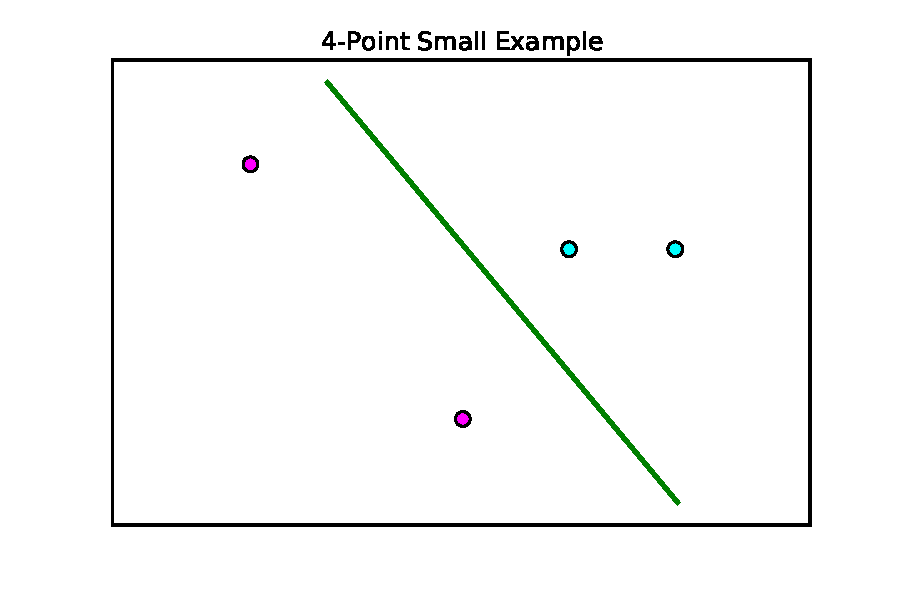
\includegraphics[width=\textwidth]{exercise1-1.pdf}
	\caption{Decision boundary for 4 points using CVXOPT and SVM with slack variables}
	\label{fig:1-1}
\end{figure}

Setting $C = 1$, 

\begin{figure}[!ht]
	\centering
	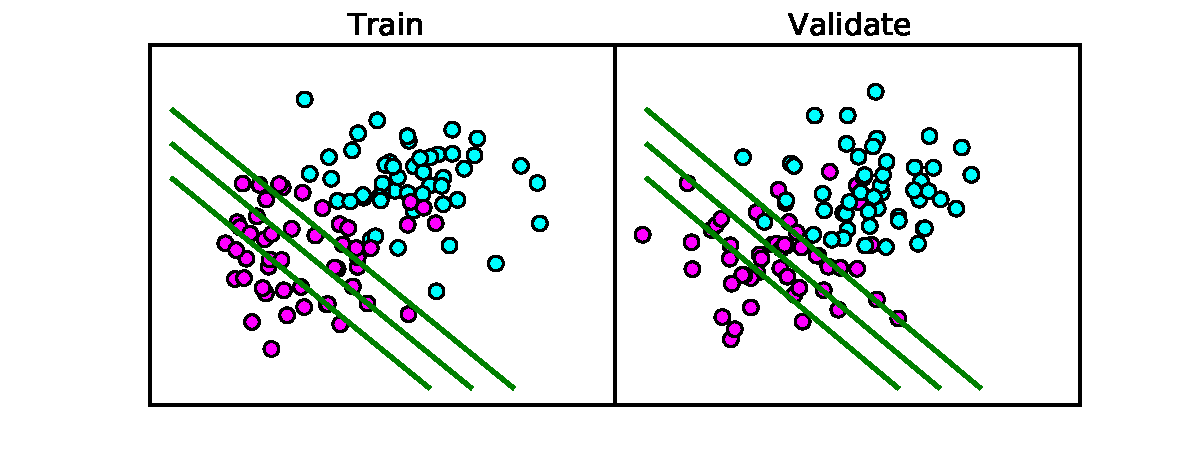
\includegraphics[width=\textwidth]{1-2-smallOverlap.pdf}
	\caption{smallOverlap}
	\label{fig:1-2-smalloverlap}
\end{figure}

\begin{figure}[!ht]
	\centering
	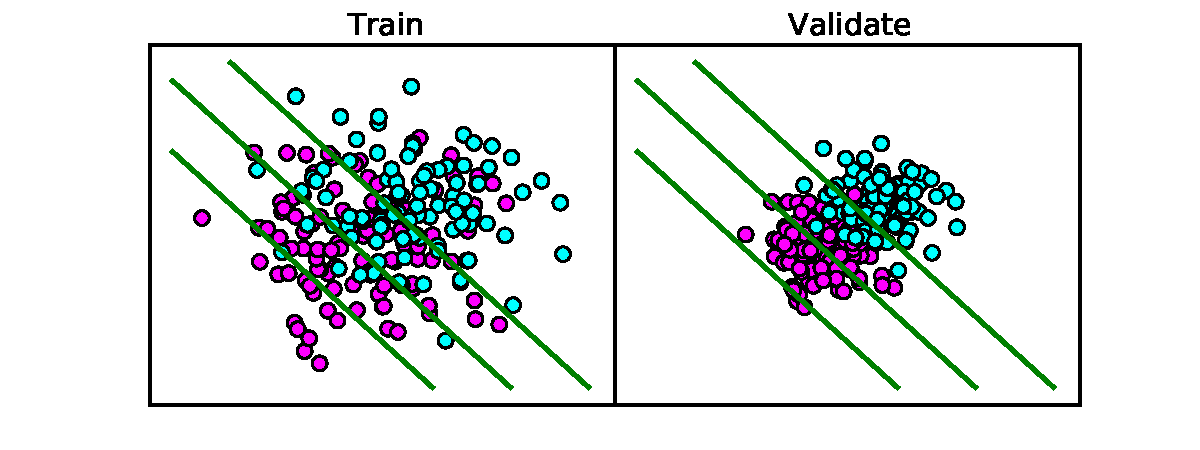
\includegraphics[width=\textwidth]{1-2-bigOverlap.pdf}
	\caption{bigOverlap}
	\label{fig:1-2-bigoverlap}
\end{figure}

\begin{figure}[!ht]
	\centering
	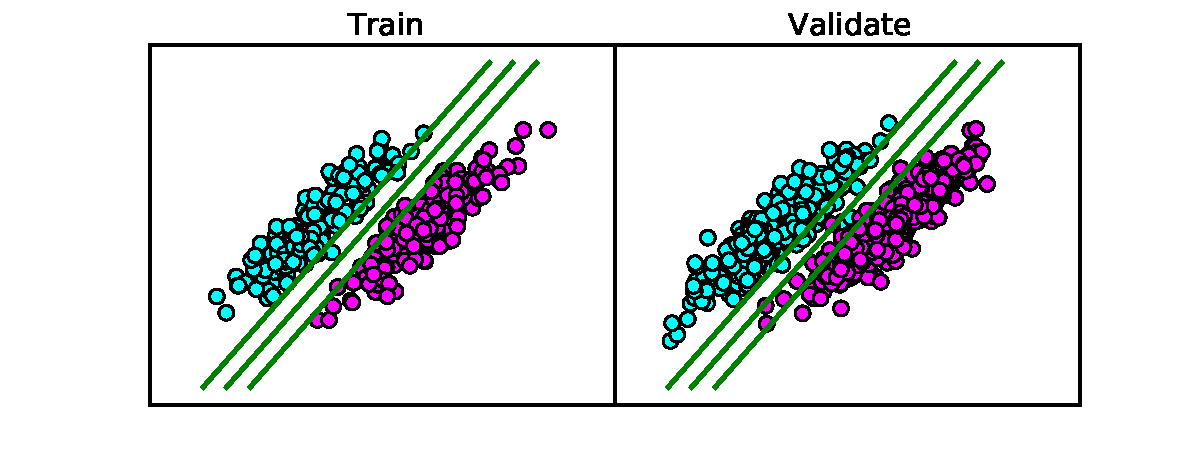
\includegraphics[width=\textwidth]{1-2-ls.pdf}
	\caption{ls}
	\label{fig:1-2-ls}
\end{figure}

\begin{figure}[!ht]
	\centering
	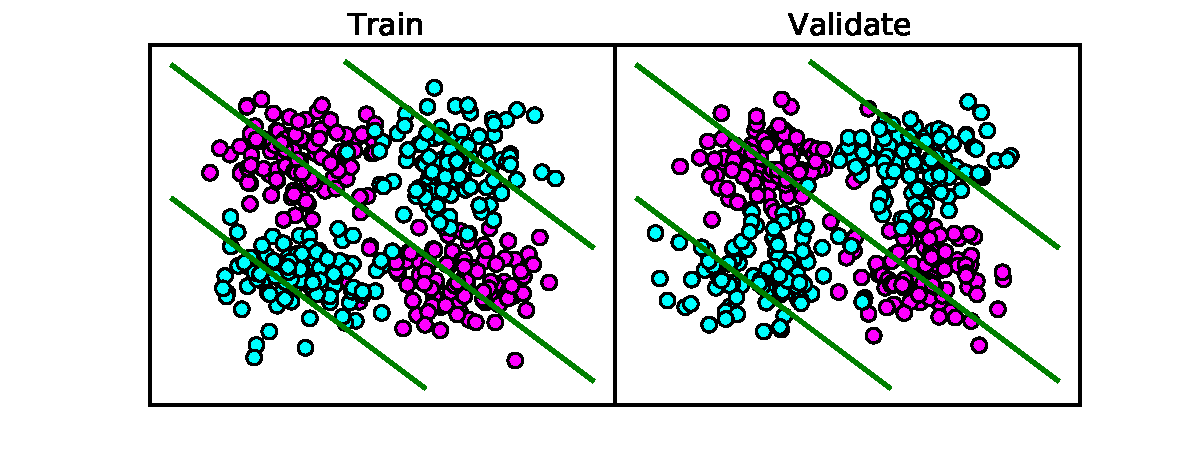
\includegraphics[width=\textwidth]{1-2-nonSep2.pdf}
	\caption{nonSep2}
	\label{fig:1-2-nonSep2}
\end{figure}

The error rates for the training and validation sets for different data sets is shown in Table \ref{tbl:1-2-error}. If a data set did not come with a training / validation set pair, the dataset was randomly cut in half for each class to use as training and validation. In general, the more separable the data set is, the better the slack-variable SVM without a regularizer does. In the non-separable case, depending on the nature of the inseparability, the solution has a higher error rate.

\begin{table}
\centering
\begin{tabular}{r|c|c}
	& Training & Validation \\ \hline
	smallOverlap & $.24$ & $.24$ \\
	bigOverlap & $.305$ & $.255$ \\
	ls & $0$ & $0.00375$ \\
	nonSep2 & $.485$ & $.495$ 
\end{tabular}
\caption{Error rates for training and validation sets, $C = 1$, linear kernel}
\label{tbl:1-2-error}
\end{table}

\begin{table}
\centering
\begin{tabular}{c|c|c|c|c|c}
Dataset 	 &	 $C$  & Geometric Margin & Support Vectors & Training & Validation \\ \hline
smallOverlap & $0.01$ 	& $1.79$		& 70 		& $.26$ & $.25$ \\
			& $0.1$		& $.93$			& 37		& $.25$ & $.24$ \\
			& $1$		& $.57$			& 24		& $.24$ & $.24$ \\
			& $10$		& $.5611$		& 22 		& $.25$ & $.24$ \\
			& $100$ 	& $.5613$		& 23		& $.25$ & $.24$ \\
bigOverlap & $0.01$ 	& $2.38$		& 148 		& $.30$ & $.25$ \\
			& $0.1$		& $1.93$		& 131		& $.31$ & $.26$ \\
			& $1$		& $1.88$		& 128		& $.31$ & $.26$ \\
			& $10$		& $1.88$		& 128 		& $.31$ & $.26$ \\
			& $100$ 	& $1.88$		& 129		& $.31$ & $.26$ \\
ls 			& $0.01$ 	& $.939$		& 177		& $.02$ & $.02$ \\
			& $0.1$		& $.48 $		& 56		& $0  $ & $.005$ \\
			& $1$		& $.31$	 		& 13		& $0  $ & $.004$ \\
			& $10$		& $.23$			& 3 		& $0 $ & $.005$ \\
			& $100$ 	& $.23$			& 31		& $0 $ & $.005$ \\
nonSep2 	& $0.01$ 	& $3.98$		& 399 		& $.48$ & $.50$ \\
			& $0.1$		& $3.37$		& 393		& $.49$ & $.50$ \\
			& $1$		& $3.29$		& 392		& $.49$ & $.50$ \\
			& $10$		& $3.29$		& 392		& $.49$ & $.50$ \\
			& $100$ 	& $3.29$		& 393		& $.49$ & $.49$ \\
\end{tabular}
\caption{Error rates for training and validation sets with varying $C$, linear kernel}
\label{tbl:1-3-linear}
\end{table}


\begin{table}
\centering
\begin{tabular}{c|c|c|c}

\end{tabular}
\caption{Error rates for training and validation sets with varying $C$, gaussian kernel}
\label{tbl:1-3-gaussian}
\end{table}

\begin{figure}[!ht]
	\centering
	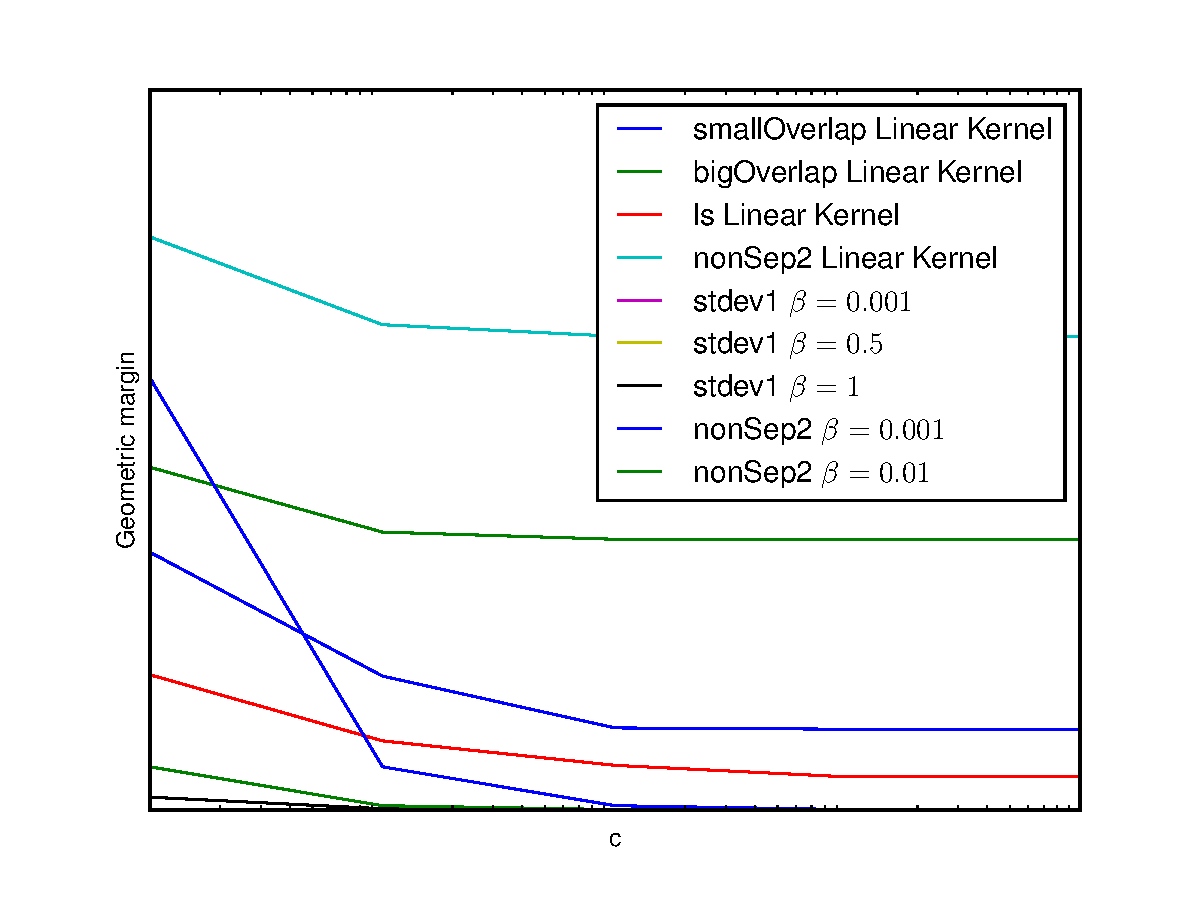
\includegraphics[width=\textwidth]{1-3-c-margin.pdf}
	\caption{Plot of the geometric margin as a function of $c$ for various kernels and datasets}
	\label{fig:1-3-c-margin}
\end{figure}

\begin{figure}[!ht]
	\centering
	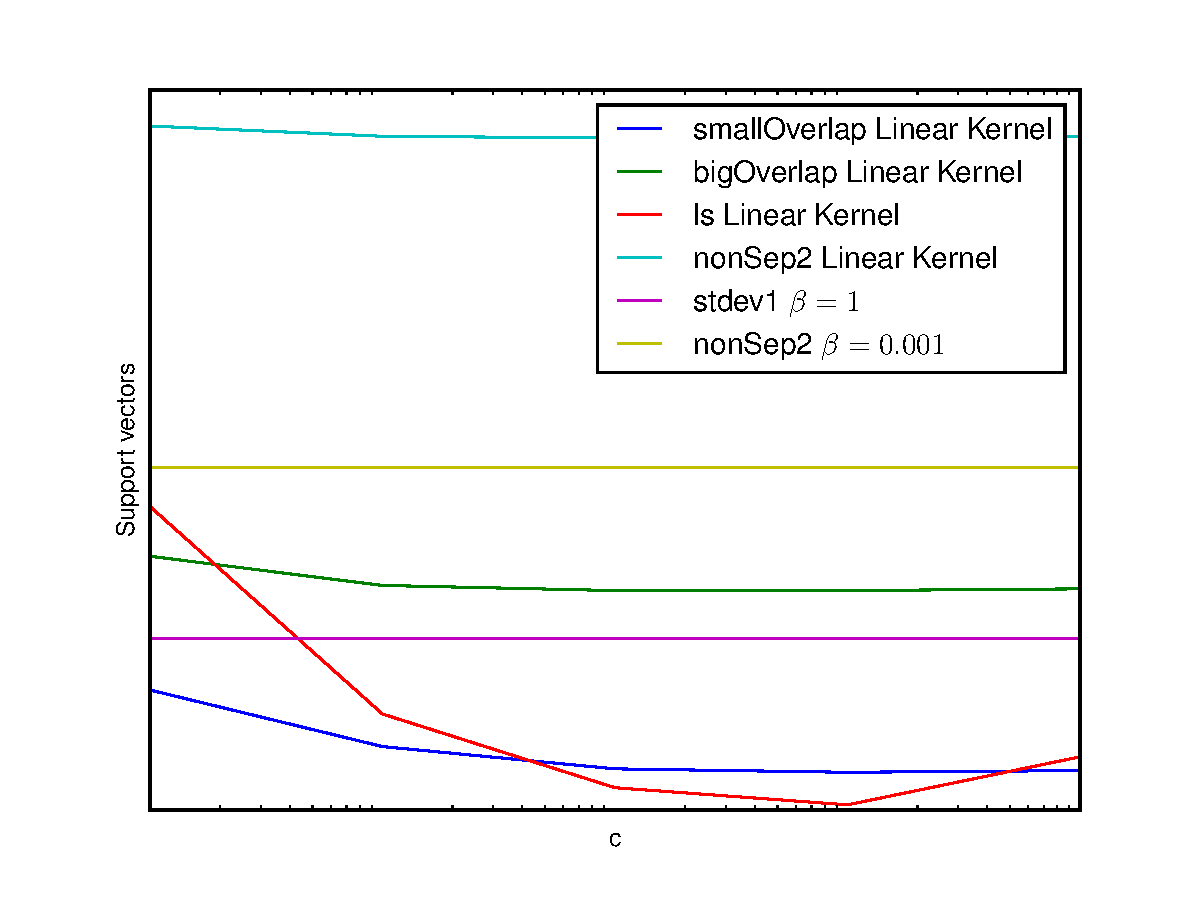
\includegraphics[width=\textwidth]{1-3-support-vectors.pdf}
	\caption{Plot of the number of support vectors as a function of $c$ for various kernels and datasets}
	\label{fig:1-3-support-vectors}
\end{figure}

As the $C$ increases, the geometric margin decreases, as shown for various values of $C$, various kernels, and various datasets in Figure \ref{fig:1-3-c-margin}. This always happens as $C$ increases, because this means there can be more slack in the final SVM, which means the SVM will be more tolerable to incorrect classifications for inseparable data. The number of support vectors decreases as $C$ increases, as shown in Figure \ref{fig:1-3-support-vectors}. This means that the classifier is less overfit on the training data and will have smaller errors on the testing data. Choosing $C$ for maximizing the margin will yield a value of $C$ equal to zero, which is the same as having a hard-margin SVM that does not perform well on non-separable data. An alternate criteria for choosing $C$ could be the minimum testing error. 

\section{Exercise 2: Logistic Regression}

2.2: 
* do training set over some values of lambda
* use that to pick lambda
* test on `validation' data and report an error value

2.3:
will need to plot lambda versus sparsity

2.4:
* do training set over some values of bandwidth with lambda = 0
* do validation set over some values of lambda
* test on test and report results

2.5:
* will need to think about this a little bit more.

3.1:
* https://piazza.com/class/hzdfawvtilo7hf?cid=434
* L2 regularization, linear case
* http://blog.datumbox.com/machine-learning-tutorial-the-multinomial-logistic-regression-softmax-regression/

* maybe need to save coefficients or predictions or something?

3.1 - LR:
* 2 features, 100 pts, 2 classes, l = 0.01 -> error = .485
* might need to randomly select subsets of data points

* bigOverlap - error is .26 on test, ,.305 on training with l = 0.1
* smallOverlap - error is .26 on test, .27 on training with l = 0.1

* tips for getting numerics to work better:
	* normalize data beforehand (then don't forget to re-normalize later)
	* 

3.2 - multiclass SVM:
* used http://scikit-learn.org/stable/modules/generated/sklearn.svm.LinearSVC.html
* can do this SO FAST it doesn't even make sense to try to do this by myself.
* tried an array of l values with L1 loss (multiclasssvm.py), best L with random partitioning of data into 3 sets. rigorous stopping criteria
* hinge loss, l2 regularization: 
	* validation error: .187
	* test error: .261
	* l: 0.01
* squared loss, l1 regularization:
	* validation error: .143
	* test error: .143
	* l: 7e-7

\end{document}